\documentclass{beamer}
\usepackage{tikz}
\usetikzlibrary{calc,arrows.meta,patterns}
\usepackage{xcolor}
\usepackage{multicol}
\usepackage{amsmath}

\title{Averages: Mean \& Median}
\author{}
\date{}

% Lego tower: \legotower{x-offset}{height}{colour}
% Each brick is 0.65 wide x 0.55 tall, with two studs
\newcommand{\legotower}[3]{%
  \foreach \i in {1,...,#2}{%
    \draw[fill=#3!55, draw=#3!80!black, line width=0.35pt]
      (#1, {(\i-1)*0.55}) rectangle (#1+0.65, {\i*0.55});
    \draw[fill=#3!80, draw=#3!80!black, line width=0.2pt]
      (#1+0.15,{(\i-1)*0.55+0.38}) circle (0.08);
    \draw[fill=#3!80, draw=#3!80!black, line width=0.2pt]
      (#1+0.44,{(\i-1)*0.55+0.38}) circle (0.08);
  }%
}

\begin{document}

\frame{\titlepage}

%------------------------------------------------
% STARTER 1
%------------------------------------------------
\begin{frame}{Starter}
\vspace{-0.8em}
\begin{columns}[T]

\column{0.33\textwidth}
\begin{center}

% Diagram 1: towers 1,3,2  (scale 0.9, bricks 0.5 tall)
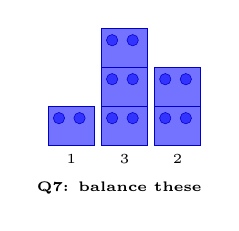
\begin{tikzpicture}[scale=0.9]
  \legotower{0.00}{1}{blue}
  \legotower{0.75}{3}{blue}
  \legotower{1.50}{2}{blue}
  \node[below,font=\tiny] at (0.325,0) {1};
  \node[below,font=\tiny] at (1.075,0) {3};
  \node[below,font=\tiny] at (1.825,0) {2};
  \node[below,font=\tiny\bfseries] at (1.0,{-0.38})
    {\textbf{Q7}: balance these};
\end{tikzpicture}

\vspace{0.55em}

% Diagram 2: towers 1,3,5,3,3  (scale 0.78 to fit width)
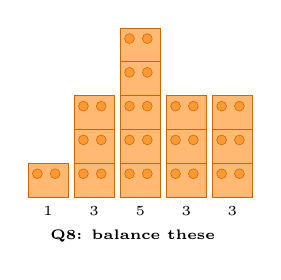
\begin{tikzpicture}[scale=0.78]
  \legotower{0.00}{1}{orange}
  \legotower{0.75}{3}{orange}
  \legotower{1.50}{5}{orange}
  \legotower{2.25}{3}{orange}
  \legotower{3.00}{3}{orange}
  \node[below,font=\tiny] at (0.325,0) {1};
  \node[below,font=\tiny] at (1.075,0) {3};
  \node[below,font=\tiny] at (1.825,0) {5};
  \node[below,font=\tiny] at (2.575,0) {3};
  \node[below,font=\tiny] at (3.325,0) {3};
  \node[below,font=\tiny\bfseries] at (1.7,{-0.38})
    {\textbf{Q8}: balance these};
\end{tikzpicture}

\end{center}

\column{0.67\textwidth}
\footnotesize
\vspace{0.2em}
\begin{enumerate}\itemsep1pt
  \begin{multicols}{2}
    \item $12 \div 4 = \mathord{?}$
    \item $18 \div 3 = \mathord{?}$
  \end{multicols}
  \begin{multicols}{2}
    \item $15 \div 3 = \mathord{?}$
    \item $28 \div 4 = \mathord{?}$
  \end{multicols}
  \item Four friends share 20 sweets equally. How many do they each get?
  \item Three children have 2, 5 and 8 stickers. They combine them and share them equally. How many does each child get?
  \item Six children have 3, 5, 3, 7, 5, 7 stickers. \textit{Estimate} the fair share, then calculate. How close were you?
  \item Draw a picture of the top towers (left), balanced to the same height without changing the total number of bricks.
  \item Draw a picture of the bottom towers (left), balanced to the same height without changing the total number of bricks.
\end{enumerate}

\end{columns}
\end{frame}

%------------------------------------------------
% STARTER 2
%------------------------------------------------
\begin{frame}{Starter}
\vspace{-0.8em}
\begin{columns}[T]

\column{0.33\textwidth}
\begin{center}

% Diagram 1: towers 3,5,4,8 — brick height 0.42 to keep 8-tower in frame
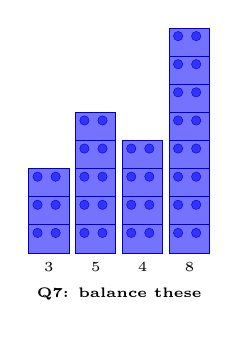
\begin{tikzpicture}[scale=0.85]
  \newcommand{\lego}[3]{%
    \foreach \ii in {1,...,#2}{%
      \draw[fill=#3!55,draw=#3!80!black,line width=0.3pt]
        (#1,{(\ii-1)*0.42}) rectangle (#1+0.6,{\ii*0.42});
      \draw[fill=#3!80,draw=#3!80!black,line width=0.15pt]
        (#1+0.13,{(\ii-1)*0.42+0.30}) circle (0.07);
      \draw[fill=#3!80,draw=#3!80!black,line width=0.15pt]
        (#1+0.40,{(\ii-1)*0.42+0.30}) circle (0.07);
    }%
  }
  \lego{0.00}{3}{blue}
  \lego{0.70}{5}{blue}
  \lego{1.40}{4}{blue}
  \lego{2.10}{8}{blue}
  \node[below,font=\tiny] at (0.30,0) {3};
  \node[below,font=\tiny] at (1.00,0) {5};
  \node[below,font=\tiny] at (1.70,0) {4};
  \node[below,font=\tiny] at (2.40,0) {8};
  \node[below,font=\tiny\bfseries] at (1.35,{-0.38})
    {\textbf{Q7}: balance these};
\end{tikzpicture}

\vspace{0.45em}

% Diagram 2: towers 1,5,2,8,4
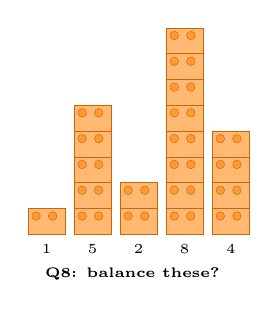
\begin{tikzpicture}[scale=0.78]
  \newcommand{\legob}[3]{%
    \foreach \ii in {1,...,#2}{%
      \draw[fill=#3!55,draw=#3!80!black,line width=0.3pt]
        (#1,{(\ii-1)*0.42}) rectangle (#1+0.6,{\ii*0.42});
      \draw[fill=#3!80,draw=#3!80!black,line width=0.15pt]
        (#1+0.13,{(\ii-1)*0.42+0.30}) circle (0.07);
      \draw[fill=#3!80,draw=#3!80!black,line width=0.15pt]
        (#1+0.40,{(\ii-1)*0.42+0.30}) circle (0.07);
    }%
  }
  \legob{0.00}{1}{orange}
  \legob{0.75}{5}{orange}
  \legob{1.50}{2}{orange}
  \legob{2.25}{8}{orange}
  \legob{3.00}{4}{orange}
  \node[below,font=\tiny] at (0.30,0) {1};
  \node[below,font=\tiny] at (1.05,0) {5};
  \node[below,font=\tiny] at (1.80,0) {2};
  \node[below,font=\tiny] at (2.55,0) {8};
  \node[below,font=\tiny] at (3.30,0) {4};
  \node[below,font=\tiny\bfseries] at (1.7,{-0.38})
    {\textbf{Q8}: balance these?};
\end{tikzpicture}

\end{center}

\column{0.67\textwidth}
\footnotesize
\vspace{0.2em}
  \begin{multicols}{2}
  \begin{enumerate}
    \item $7 \times 8 = \mathord{?}$
    \item $63 \div 7 = \mathord{?}$
    \end{enumerate}
  \end{multicols}
  \begin{multicols}{2}
  \begin{enumerate}
  \setcounter{enumi}{2}
    \item $48 \div 8 = \mathord{?}$
    \item $5 \times 9 = \mathord{?}$
    \end{enumerate}
  \end{multicols}
  \begin{enumerate}
  \setcounter{enumi}{4}
  \item Five children have 4, 7, 3, 6, 5 marbles. Shared equally, how many each?
  \item Six friends earn £8, £14, £10, £6, £12, £10 at a car wash. Split fairly — how much each?
  \item Eight runners finish in 54, 48, 61, 57, 50, 63, 55, 52 s. Without doing any calculations, estimate the average time.
  \item What heights would the top towers balance out to?
  \item What heights would the bottom towers balance out to?
\end{enumerate}

\end{columns}
\end{frame}

%------------------------------------------------
% STARTER 3
%------------------------------------------------
\begin{frame}{Starter}
\vspace{-0.8em}

\footnotesize
\vspace{0.2em}
\begin{enumerate}\itemsep1pt
  \begin{multicols}{2}
    \item $3 + 4 + 7 = \mathord{?}$
    \item $15+27+18=\mathord{?}$
    \item $60\div 4=\mathord{?}$
    \item $-15 \div 3=\mathord{?}$
  \end{multicols}
  \vspace{-1em}
  \item What is the mean of: $4,\ 6,\ 2,\ 8$
  \item What is the mean  of: $3,\ 9,\ 5,\ 7,\ 1$
  \item What is the mean  of: $-3,\ 5,\ -1,\ 7,\ 2$
  \item What is the mean  of: $-8,\ -2,\ -5,\ -1,\ -4$
\end{enumerate}

\begin{enumerate}\itemsep1pt
  \setcounter{enumi}8
  \item The mean of four numbers is 9. Three are 6, 11 and 8. Find the fourth.
  \item The mean of $3,\ 7,\ x,\ 10$ is $8$. What is $x$?
\end{enumerate}


\end{frame}

%------------------------------------------------
% STARTER 4
%------------------------------------------------
\begin{frame}{Starter 4}
\vspace{-0.8em}
\begin{columns}[T]

\column{0.33\textwidth}
\begin{center}


\vspace{7em}

% Dot plot: house prices with outlier
\begin{tikzpicture}[scale=0.72]
  \draw[thick,->] (-0.2,0) -- (4.6,0);
  \foreach \xd in {0.3, 0.55, 0.8, 1.05, 1.3}{
    \fill[blue] (\xd,0.22) circle (0.1);
  }
  \fill[red] (4.2,0.22) circle (0.1);
  \node[below,font=\tiny,blue] at (0.8,{-0.1})  {£125--140k};
  \node[below,font=\tiny,red]  at (4.2,{-0.1})  {£980k};
  \draw[<->,dashed,gray] (1.35,0.52) -- (4.1,0.52)
    node[midway,above,font=\tiny,gray]{big gap};
  \node[below,font=\tiny\bfseries] at (2.1,{-0.55})
    {\textbf{Q10}: house prices on a road}
\end{tikzpicture}

\end{center}

\column{0.67\textwidth}
\footnotesize
\vspace{0.2em}
\begin{enumerate}\itemsep1pt
  \begin{multicols}{2}
    \item $4+2+10=\mathord{?}$
    \item $-4+9 = \mathord{?}$
    \item $-3-5 = \mathord{?}$
    \item $6 \times 4 = \mathord{?}$
  \end{multicols}
  \item Order smallest to largest: $8,3,11,5,7$. Which is the middle value?
  \item Order: $21,14,9,35,17,28,6$. Which is the middle value?
  \item For $3,7,8,9,41$: \textit{estimate} whether the middle value is above or below the mean. Then check.
  \item What is the middle value of: $-7,\ -2,\ -5,\ 1,\ -1,\ 3,\ -3$
  \item What is the middle value of: $\tfrac{1}{2},\ \tfrac{1}{4},\ \tfrac{3}{4},\ \tfrac{1}{8},\ \tfrac{5}{8}$.
  \item House prices on a road are: £130k, £125k, £140k, £128k, £135k, \textcolor{red}{£980k}. Why might the mean not be helpful?
\end{enumerate}

\end{columns}
\end{frame}

%------------------------------------------------
% STARTER 5
%------------------------------------------------
\begin{frame}{Starter}
\vspace{-0.8em}
\begin{columns}[T]

\column{0.33\textwidth}
\begin{center}

\vspace{7em}

% Dot plot showing mean pulled by outlier vs stable median
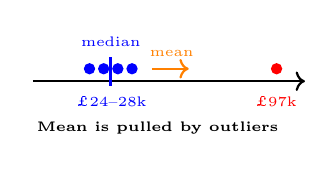
\begin{tikzpicture}[scale=0.72]
  \draw[thick,->] (-0.2,0) -- (4.6,0);
  \foreach \xd in {0.8, 1.05, 1.3, 1.55}{
    \fill[blue] (\xd,0.22) circle (0.1);
  }
  \fill[red] (4.1,0.22) circle (0.1);
  \node[below,font=\tiny,blue] at (1.2,{-0.1})  {£24--28k};
  \node[below,font=\tiny,red]  at (4.1,{-0.1})  {£97k};
  \draw[blue,very thick] (1.175,0.42) -- (1.175,-0.08);
  \node[above,blue,font=\tiny] at (1.175,0.44) {median};
  \draw[->,thick,orange] (1.9,0.22) -- (2.55,0.22);
  \node[above,orange,font=\tiny] at (2.25,0.26) {mean};
  \node[below,font=\tiny\bfseries] at (2.0,{-0.55})
    {Mean is pulled by outliers};
\end{tikzpicture}

\vspace{0.5em}


\end{center}

\column{0.67\textwidth}
\footnotesize
\vspace{0.3em}
\begin{enumerate}\itemsep1pt
  \begin{multicols}{2}
    \item $-6+(-2) = \mathord{?}$
    \item $\frac{1}{3}+\frac{1}{2} = \mathord{?}$
  \end{multicols}
  \vspace{-1em}
  \item Median of: $3,\ 9,\ 4,\ 7,\ 1$
  \item Mean \textbf{and} median of: $5,\ 8,\ 3,\ 12,\ 7$. Which is larger?
  \item Five salaries are: £24k, £26k, £25k, £28k, \textcolor{red}{£97k}. Would you prefer to use the mean or the median to find the average?
  \item For $-10,-1,0,2,3$: \textit{estimate} whether the mean is positive or negative. Then calculate both mean and median.
  \item Find the mean and median of: $-6,\ -2,\ 4,\ -3,\ 7,\ 0$
  \item What is the median of: $\frac{1}{3},\ \frac{3}{4},\ \frac{1}{2},\ \frac{1}{6},\ \frac{2}{3},\ \frac{1}{4}$
  \item True or False?\\
    (a) The median is always one of the values in the dataset.\\
    (b) The mean and median are always different.\\
    (c) A very large outlier affects the median more than the mean.

\end{enumerate}

\end{columns}
\end{frame}

\end{document}